\documentclass[11pt]{article}
\usepackage[margin=1in]{geometry}
\usepackage{amsmath}
\usepackage{graphicx}
\usepackage{tikz-cd}
\usepackage{multicol}

\setlength{\parindent}{0pt}
\setlength{\parskip}{1\baselineskip}

\begin{document}

\section*{What is Prism?}

\textbf{Prism} is an AI-powered \LaTeX{} editor for writing scientific documents. It supports real-time collaboration with coauthors and includes OpenAI-powered intelligence to help you draft and edit text, reason through ideas, and handle formatting.

\section*{Features}

\begin{multicols}{2}
Prism includes ChatGPT directly in the editor and can access your project, so you can ask it to do things like:

``Add the equation for the Laplace transform of $t\cos(at)$ to the introduction.''
\[
  \mathcal{L}\left\{ t \cos(a t) \right\} = \frac{ s^2 - a^2 }{ (s^2 + a^2)^2 }
\]

``Add a 4-by-4 table'' to the summary section.
\begin{center}
\resizebox{0.5\linewidth}{!}{%
\begin{tabular}{|c|c|c|c|}
  \hline
  1 & 2 & 3 & 4 \\
  \hline
  5 & 6 & 7 & 8 \\
  \hline
  9 & 10 & 11 & 12 \\
  \hline
  13 & 14 & 15 & 16 \\
  \hline
\end{tabular}%
}
\end{center}

``Proofread this and highlight any errors or gaps in logic, and make suggestions for how I can improve the clarity of the section.''

``Are there any corollaries or follow-on implications of Theorem 3.1 that I've missed? Are all the bounds tight, or can some be relaxed?''

\columnbreak

``Write an abstract based on the rest of the paper''

``Add a bibliography to my paper, and suggest related work I may have missed.''

``Generate this hand-drawn diagram in \LaTeX{}.''
\par\noindent
\begin{minipage}[t]{0.49\linewidth}
  \vspace{0pt}
  \centering
  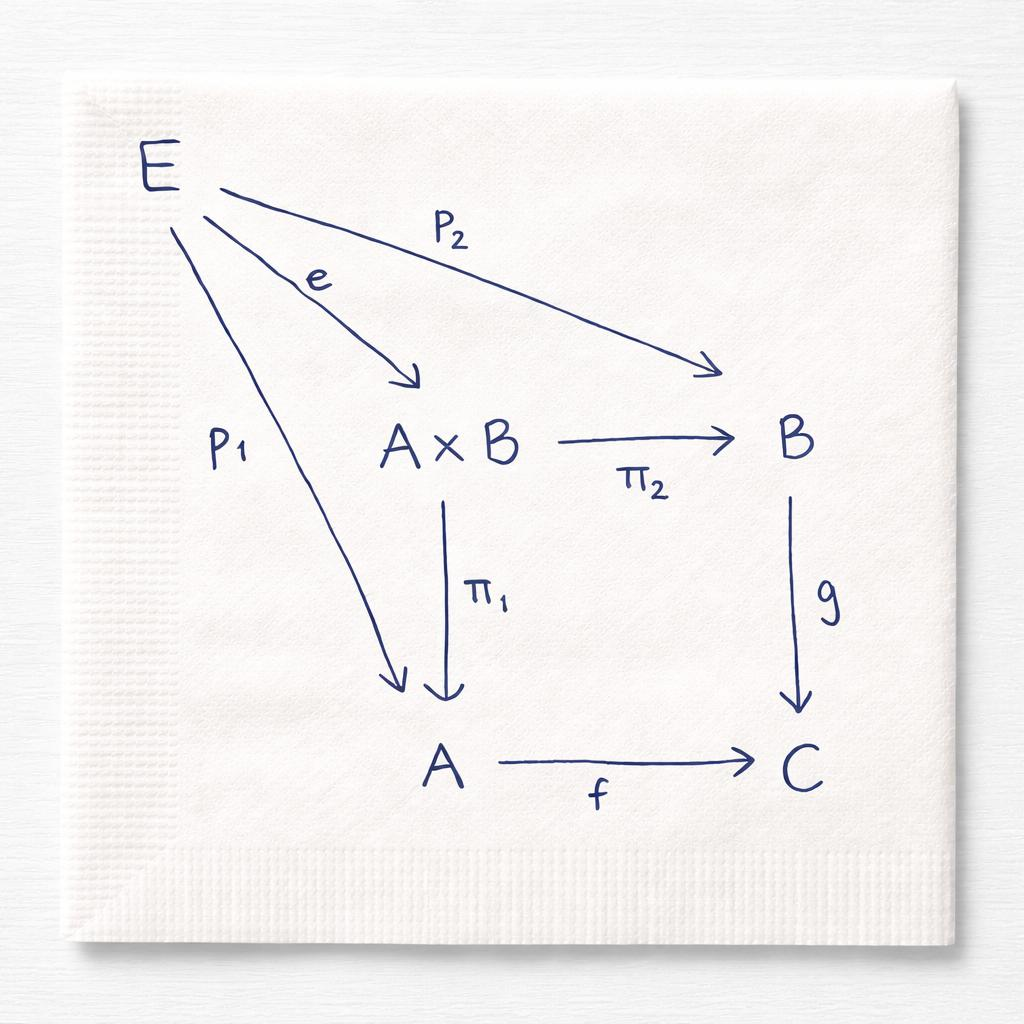
\includegraphics[width=\linewidth]{diagram.jpg}
\end{minipage}\hfill
\begin{minipage}[t]{0.49\linewidth}
  \vspace{0pt}
  \centering
  \resizebox{\linewidth}{!}{$
    \begin{tikzcd}[row sep=2em, column sep=1.5em, ampersand replacement=\&]
      E
        \arrow[dr, "e"']
        \arrow[drr, "p_2"]
        \arrow[ddr, "p_1"']
      \& \& \\
      \& A \times B \arrow[r, "\pi_2"'] \arrow[d, "\pi_1"] \& B \arrow[d, "g"] \\
      \& A \arrow[r, "f"'] \& C
    \end{tikzcd}
  $}
\end{minipage}
\par

``Add any missing dependencies across my project.''

``Generate a 200-word summary for a popular audience, in German.''

``Generate a Beamer presentation with each slide in its own file.''
\end{multicols}

\section*{Collaboration}

Invite collaborators by clicking the ``Share'' menu. As you edit, they will see your updates in real time. You can also leave comments by highlighting text and selecting "Leave a comment."

\end{document}